\documentclass[10pt,pdf,utf8,russian,aspectratio=169]{beamer}
\usepackage[T2A]{fontenc}
\usetheme{Singapore}
\usepackage{setspace}
\usepackage{amsmath}
\usepackage{pgfplots}
\usepackage[utf8]{inputenc}
\usepackage{tikz-cd}
\usepackage[all, 2cell]{xy}
\usepackage{amssymb}
\usepackage{verba tim}
\usepackage[all]{xy}
\usepackage{tikz}
\usepackage{bussproofs}
\usepackage{dsfont}
\usepackage{mathabx}
\usepackage{animate}
\usetikzlibrary{graphs}
\usetikzlibrary{arrows}
\usepackage{hyperref}
\usepackage[english,russian]{babel}
\usepackage{listings}
\usepackage{color}
\usepackage{tikz}
\usepackage{listings}
\pgfplotsset{compat=1.16}
\newtheorem{defin}{Definition}
\newtheorem{theor}{Theorem}
\newtheorem{prop}{Proposition}
\title{Functional programming, Seminar No. 3}
\author{Danya Rogozin \\ Lomonosov Moscow State University, \\ Serokell O\"{U}}
\date{Higher School of Economics \\ Faculty of Computer Science}
\begin{document}
\lstset{
  frame=none,
  xleftmargin=2pt,
  stepnumber=1,
  numbers=left,
  numbersep=5pt,
  numberstyle=\ttfamily\tiny\color[gray]{0.3},
  belowcaptionskip=\bigskipamount,
  captionpos=b,
  escapeinside={*'}{'*},
  language=haskell,
  tabsize=2,
  emphstyle={\bf},
  commentstyle=\it,
  stringstyle=\mdseries\rmfamily,
  showspaces=false,
  keywordstyle=\bfseries\rmfamily,
  columns=flexible,
  basicstyle=\small\sffamily,
  showstringspaces=false,
  morecomment=[l]\%,
}
\maketitle

\begin{frame}
  \frametitle{Intro}

  On the previous seminar, we
  \onslide<1->{
  \begin{itemize}
    \item studied the basic Haskell syntax
    \item introduced the notion of a weak head normal form to describe the operatonal semantics of Haskell
    \item analysed the regrettable cicrumstances according to which Haskell doesn't have the Church-Rosser property as a system of typed lambda calculus
  \end{itemize}
  }

\vspace{\baselineskip}

\onslide<2->{
Today we
  \begin{itemize}
    \item investigate the Haskell type system more deeply and overview the advantages of parametric polymorphism
    \item take a look at bounded polymorphism and discuss type classes
  \end{itemize}
  }
\end{frame}

\begin{frame}[fragile]
  \frametitle{Motivation}
  Let us recall the example of a higher order function from the previous seminar:

  \begin{lstlisting}[language=Haskell]
  changeTwiceBy :: (Int -> Int) -> Int -> Int
  changeTwiceBy operation value = operation (operation value)
  \end{lstlisting}

  \vspace{\baselineskip}

  It is clear that one may implement the function for Boolean values and strings that have the same behaviour as the function above:

  \begin{lstlisting}[language=Haskell]
  changeTwiceByBool :: (Bool -> Bool) -> Bool -> Bool
  changeTwiceByBool operation value = operation (operation value)

  changeTwiceByString :: (String -> String) -> String -> String
  changeTwiceByString operation value = operation (operation value)
  \end{lstlisting}

  \onslide<2->{
  One needs to have a way to avoid such a boilerplate.
  }
\end{frame}

\begin{frame}[fragile]
  \frametitle{Parametric polymorphism}

  The key idea of parametric polymorphism that the same function might be called on distinct data types. Here are the initial polymorphic examples:

  \begin{lstlisting}[language=Haskell]
  id :: a -> a
  id x = x

  const :: a -> b -> a
  const a b = a

  fst :: (a, b) -> a
  fst (a, b) = a

  snd :: (a, b) -> b
  snd = "guess what"

  swap :: (a, b) -> (b, a)
  swap (a, b) = (b, a)
  \end{lstlisting}
\end{frame}

\begin{frame}
  \frametitle{The meme time}

  \begin{center}
  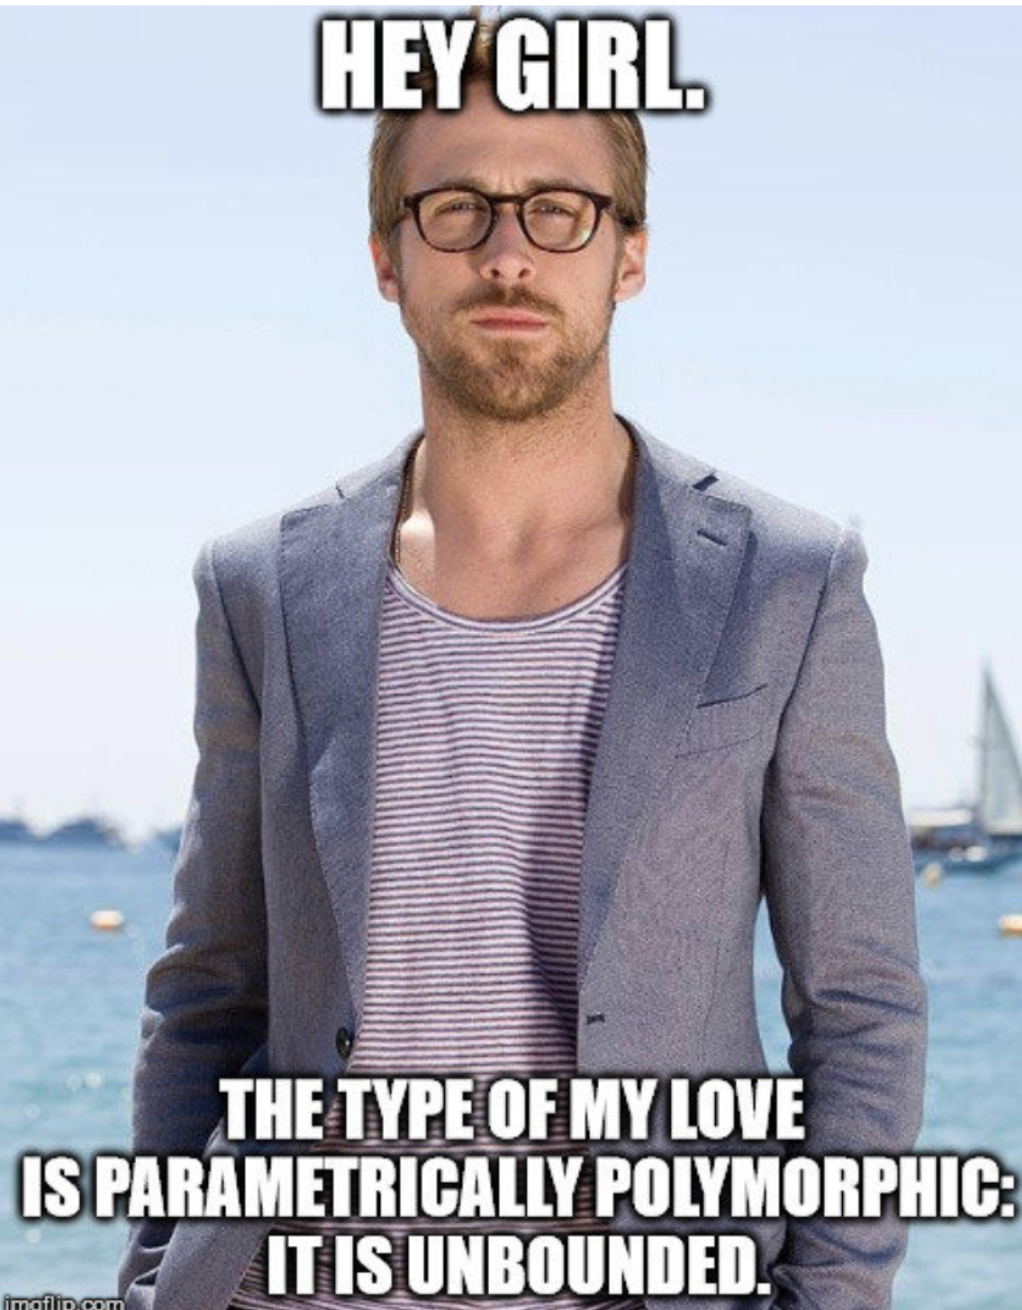
\includegraphics[scale=0.3]{Pics/Ryan.png}
  \end{center}
\end{frame}

\begin{frame}
  \frametitle{The functions above in the GHCi session}

  \begin{center}
  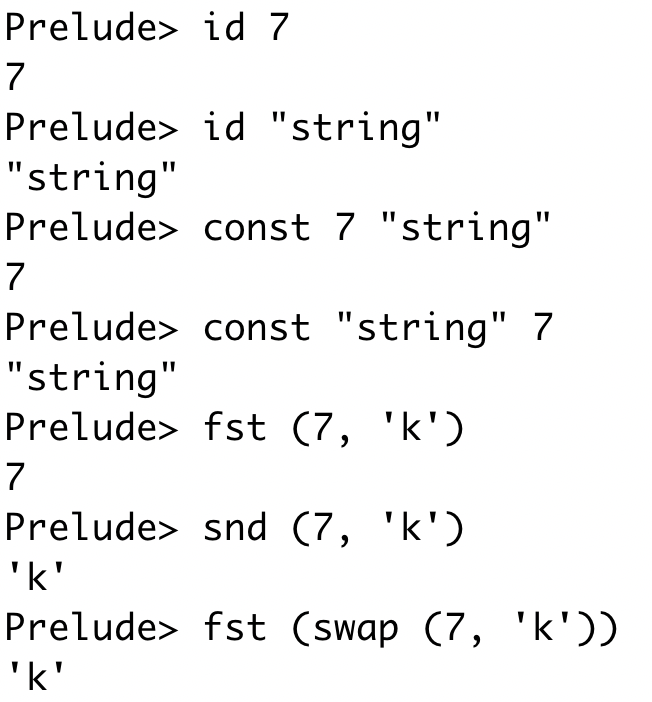
\includegraphics[scale=0.5]{Pics/Triv.png}
  \end{center}
\end{frame}

\begin{frame}[fragile]
  \frametitle{Higher order functions and parametric polymorpism}

  \begin{lstlisting}[language=Haskell]
  infixr 9 .
  (.) :: (b -> c) -> (a -> b) -> a -> c
  f . g = \x -> f (g x)

  flip :: (a -> b -> c) -> b -> a -> c
  flip f b a = f a b

  fix :: (a -> a) -> a
  fix = error "this is your homework"

  curry :: ((a, b) -> c) -> a -> b -> c
  curry f x y = f (x, y)

  uncurry :: (a -> b -> c) -> ((a, b) -> c)
  uncurry f p = f (fst p) (snd p)
  \end{lstlisting}
\end{frame}

\begin{frame}[fragile]
    \frametitle{The functions above in the GHCi session. The composition examples}

\begin{lstlisting}[language=Haskell]
incNegate :: Int -> Int
incNegate x = negate (x + 1)

incNegate x = negate $ x + 1

incNegate x = (negate . (+1)) x

incNegate x = negate . (+1) $ x

incNegate   = negate . (+1)
\end{lstlisting}
\end{frame}

\begin{frame}
  \frametitle{The functions above in the GHCi session. \verb"curry" and \verb"uncurry"}

  \begin{center}
  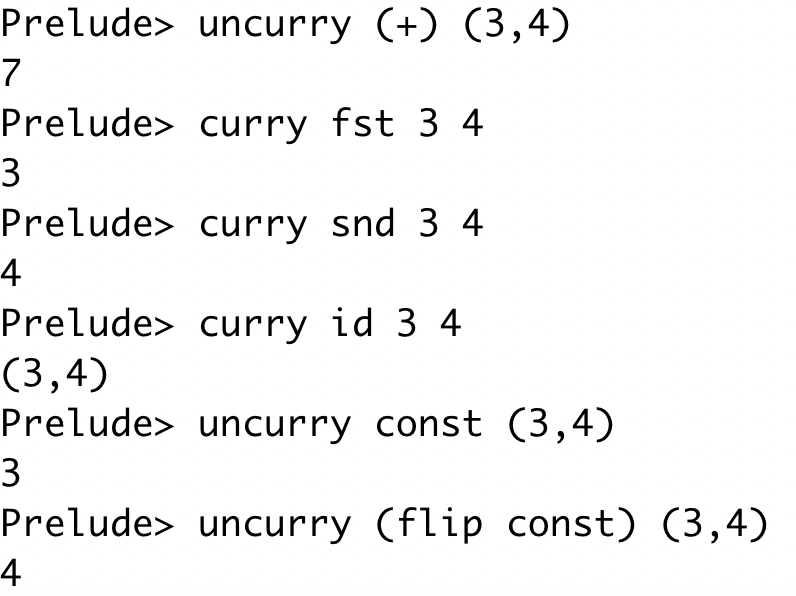
\includegraphics[scale=0.554]{Pics/Curry.png}
  \end{center}
\end{frame}

\begin{frame}[fragile]
  \frametitle{The functions above in the GHCi session. The \verb"flip" example}

  \begin{lstlisting}[language=Haskell]
  show2 :: Int -> Int -> String
  show2 x y = show x ++ " and " ++ show y

  showSnd, showFst, showFst' :: Int -> String
  showSnd  = show2 1
  showFst  = flip show2 2
  showFst' = (`show2` 2)
  \end{lstlisting}

\onslide<2->{
  \begin{center}
  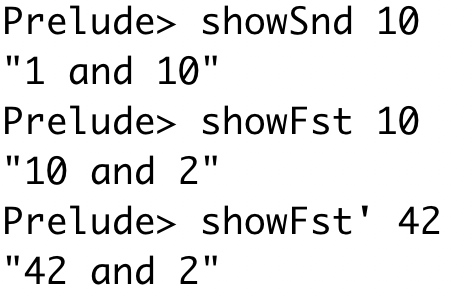
\includegraphics[scale=0.47]{Pics/Flip.png}
  \end{center}
  }
\end{frame}

\begin{frame}[fragile]
  \frametitle{Bye-bye boilerplate!}

  All these functions
  \begin{lstlisting}[language=Haskell]
  changeTwiceBy :: (Int -> Int) -> Int -> Int
  changeTwiceBy operation value = operation (operation value)

  changeTwiceByBool :: (Bool -> Bool) -> Bool -> Bool
  changeTwiceByBool operation value = operation (operation value)

  changeTwiceByString :: (String -> String) -> String -> String
  changeTwiceByString operation value = operation (operation value)
  \end{lstlisting}

  might be replaced to the following ones:
  \begin{lstlisting}[language=Haskell]
  applyTwice :: (a -> a) -> a -> a
  applyTwice f a = f (f a)

  applyTwice' :: (a -> a) -> a -> a
  applyTwice' f a = f . f $ a

  applyTwice'' :: (a -> a) -> a -> a
  applyTwice'' f = f . f
  \end{lstlisting}
\end{frame}

\begin{frame}[fragile]
  \frametitle{HOF, polymorpism, and lists}

  \begin{lstlisting}[language=Haskell]
  map     :: (a -> b)      -> [a] -> [b]

  filter  :: (a -> Bool)   -> [a] -> [a]

  zipWith :: (a -> b -> c) -> [a] -> [b] -> [c]

  length :: [a] -> Int

  \end{lstlisting}

\vspace{\baselineskip}

\onslide<2->{
  We discuss their implementations closely on the next seminar. Here we just take a look at their behaviour.
  }
\end{frame}

\begin{frame}[fragile]
    \frametitle{The composition examples + list functions}
\begin{lstlisting}[language=Haskell]
foo, bar :: [Int] -> Int
foo patak = length $ filter odd $ map (div 2) $ filter even $ map (div 7) patak
bar       = length . filter odd . map (div 2) . filter even . map (div 7)
\end{lstlisting}
\end{frame}

\begin{frame}[fragile]
    \frametitle{The composition examples + list functions}
    \begin{lstlisting}[language=Haskell]
    stringsTransform :: [String] -> [String]
    stringsTransform l = map (\s -> map toUpper s) (filter (\s -> length s == 5) l)

    stringsTransform l = map (\s -> map toUpper s) $ filter (\s -> length s == 5) l

    stringsTransform l = map (map toUpper) $ filter ((== 5) . length) l

    stringsTransform = map (map toUpper) . filter ((== 5) . length)
    \end{lstlisting}
\end{frame}

\begin{frame}
  \frametitle{Restricted strictness}
\end{frame}

\begin{frame}
  \frametitle{Bounded polymorphism and type classes}

\onslide<1->{
  The idea of bounded (ad hoc) polymorphism is that one has a general interface with instances for each concrete data type.
}

\onslide<2->{
\begin{center}
\includegraphics[scale=0.35]{Pics/NineAdHoc.png}
\end{center}
}
\end{frame}

\begin{frame}[fragile]
  \frametitle{The notion of a type class}

  \emph{A type class} is a collection of functions with type signatures with a common type parameter. The example given:

  \begin{lstlisting}[language=Haskell]
  class Eq a where
    (==) :: a -> a -> Bool
    (/=) :: a -> a -> Bool
  \end{lstlisting}

  \vspace{\baselineskip}

  A type class name introduce a constraint called \emph{context}:

  \begin{lstlisting}[language=Haskell]
  elem :: Eq a => a -> [a] -> Bool
  elem _ [] = False
  elem x (y:ys) = x == y || elem x ys
  \end{lstlisting}
\end{frame}

\begin{frame}[fragile]
  \frametitle{Instance declarations}

  A given data type \verb"a" has the \emph{instance} of a type class if every function of that class is implemented for \verb"a". The example:

  \begin{lstlisting}[language=Haskell]
  instance Eq Bool where
    True == True   = True
    False == False = True
    _ == _         = False

    x =/= y        = neg (x == y)
  \end{lstlisting}
\end{frame}

\begin{frame}[fragile]
  \frametitle{Polymorphism + instance declarations}

  A type parameter in an instance declaration might be polymorphic itself:

  \begin{lstlisting}[language=Haskell]
  instance Eq a => Eq [a] where
    []       == []       = True
    (x : xs) == (y : ys) = x == y && xs == ys
    _        == _        = False
  \end{lstlisting}
\end{frame}

\begin{frame}
  \frametitle{The \verb"Eq" type class generally}

  The \verb"Eq" type class is a type class that allows one to
\end{frame}

\begin{frame}[fragile]
  \frametitle{The \verb"Show" type class}

  \begin{lstlisting}[language=Haskell]
  class Show a where
    showsPrec :: Int -> a -> ShowS
    show :: a -> String
    showList :: [a] -> ShowS
    {-# MINIMAL showsPrec | show #-}
  \end{lstlisting}
\end{frame}

\begin{frame}[fragile]
  \frametitle{The \verb"Ord" type class}

  \begin{lstlisting}[language=Haskell]
  class Eq a => Ord a where
    compare :: a -> a -> Ordering
    (<) :: a -> a -> Bool
    (<=) :: a -> a -> Bool
    (>) :: a -> a -> Bool
    (>=) :: a -> a -> Bool
    max :: a -> a -> a
    min :: a -> a -> a
    {-# MINIMAL compare | (<=) #-}
  \end{lstlisting}
\end{frame}

\begin{frame}[fragile]
  \frametitle{The \verb"Num" type class}

  \begin{lstlisting}[language=Haskell]
  class Num a where
    (+) :: a -> a -> a
    (-) :: a -> a -> a
    (*) :: a -> a -> a
    negate :: a -> a
    abs :: a -> a
    signum :: a -> a
    fromInteger :: Integer -> a
    {-# MINIMAL (+), (*), abs, signum, fromInteger, (negate | (-)) #-}
  \end{lstlisting}
\end{frame}

\begin{frame}[fragile]
  \frametitle{The \verb"Enum" and \verb"Bounded" type classes}

\begin{lstlisting}[language=Haskell]
  class Enum a where
    succ :: a -> a
    pred :: a -> a
    toEnum :: Int -> a
    fromEnum :: a -> Int

    enumFrom :: a -> [a]
    enumFromThen :: a -> a -> [a]
    enumFromTo :: a -> a -> [a]
    enumFromThenTo :: a -> a -> a -> [a]
    {-# MINIMAL toEnum, fromEnum #-}
  \end{lstlisting}

\begin{lstlisting}[language=Haskell]
  class Bounded a where
    minBound :: a
    maxBound :: a
    {-# MINIMAL minBound, maxBound #-}
  \end{lstlisting}
\end{frame}

\begin{frame}[fragile]
  \frametitle{The \verb"Fractional" type class}

\begin{lstlisting}[language=Haskell]
  class Num a => Fractional a where
    (/) :: a -> a -> a
    recip :: a -> a
    fromRational :: Rational -> a
    {-# MINIMAL fromRational, (recip | (/)) #-}
  \end{lstlisting}
\end{frame}

\begin{frame}
  \frametitle{Summary}
\end{frame}


\end{document}
